\section{Qui bénificie du déneigement des routes}
Pour comprendre qui compose notre clientèle, il est important de comprendre à qui
bénéficie le déneigement des routes.

\begin{figure}[H]
    \centering
    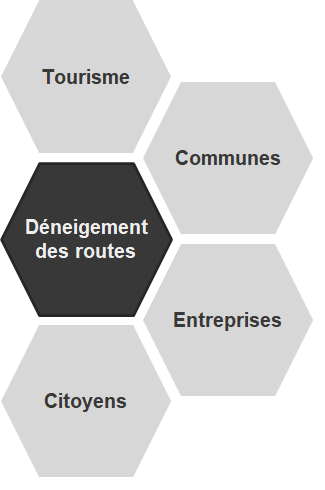
\includegraphics[width=0.25\linewidth]{Images/business/beneficiaires.png}
    \caption[]{Bénéficiaires du déneigement}
    \label{fig:beneficiaires}
\end{figure}

\begin{description}
    \item[Tourisme] \hfill \\
    Si vous êtes en vacances en station, ne pas pouvoir profiter d'une journée à ski car
    les routes ne sont pas déneigées serait le comble. C'est pourquoi tous les commerces
    et communes des régions touristiques ont besoin de route impeccables en tout temps.
    \item[Communes] \hfill \\
    Une route déneigée, c'est une route sur laquelle vous évitez des accidents dus à la neige.
    C'est une route qui ne sera pas bloquée car une voiture est à l'équerre et bloque le car postal.
    C'est la mission d'une commune d'entretenir ses routes pour assurer la sécurité de ses citoyens.
    \item[Entreprises] \hfill \\
    Un boulanger a besoin de sa livraison tôt le matin. S'il ne l'a pas reçue, il ne pourra
    pas faire son pain à temps pour ses clients du matin. Il est donc fondamental que la route
    permette au livreur d'arriver à temps.
    Un opticien, avec seulement 2 employés, peut se retrouver à ne pas pouvoir ouvrir à l'heure
    si tout le monde est coincé à cause de la neige.
    \item[Citoyens] \hfill \\    
    Personne n'a envie de passer 15 minutes à déneiger sa voiture, pour finalement trouver une
    route en piteux état.
\end{description}

\section{Analyse de la clientèle}
\subsection{Communes}
Les administrations publiques verront en ce projet la possibilité de superviser
un territoire parfois compliqué (par exemple, les fonds de vallée,
routes de montagnes, etc...) et d'efficacement déneiger ou saler
afin que la chaussée soit prête à accueillir des automobilistes dès que possible.
Par exemple, la commune d'Ayent, étant très vaste et possédant des zones
où l'accès est compliqué, fait face au problème de la répartition inhomogène
des chutes de neige. Durant la nuit, il est donc contraignant d'envoyer
quelqu'un contrôler chaque zone. Des allers-retours inutiles peuvent être
évités grâce à un réseau de capteurs.
De plus, malgré la mise en place de personnel de piquet, il est possible
d'être surpris par des chutes de neige non annoncées par la météo.

\subsection{Entreprise privée}
De nombreuses entreprises fournissent des services de déneigement pour particuliers.
Installer des capteurs chez les clients (par exemple devant un boulanger),
permettrait de mieux planifier le déneigement, et ainsi d'améliorer la qualité
du service offert aux particuliers.
Notre solution permet également de minimiser les temps de sortie des véhicules,
et ainsi réaliser des économies.
Intégrer à tous leurs clients, LoRaSnow donnera une vue d'ensemble de l'état
des routes de leurs clients, optimisant par la même occasion leur parcours.
\newpage

\section{Analyse du marché}
\subsection{Demande}
La demande pour une telle solution est déjà présente, notamment en Valais.
La commune d'Ayent a déjà fait savoir son intérêt pour ce type de détection.

\subsection{Offres présentes sur le marché}
Actuellement, aucune offre comparable directement avec la nôtre n'est disponible.

\section{Analyse des partenaires}
\subsection{Eurocircuit}
Eurocircuit, leader européen dans la production de circuits imprimés sur mesures,
partenaire de choix pour la réalisation de produits électronique.
À noter que ce partenaire propose aussi un service de montage électronique,
ce qui nous permet de faire sous-traiter cette partie compliquée pour
un coût plus faible qu'en Suisse.

\subsection{Pfefferlé Sion}
Pfefferlé serait notre fournisseur de visserie et autre quincailleries (p. ex: la grenouillère du boitier).
Leur proximité est un avantage pour réduire les coûts et alimenter l'économie locale.

\subsection{Protolabs}
Protolabs est un fabricant de moule à injection plastique. Il offre la possibilité de fabriquer des
moules pour des petites productions (env. 1000 unités).
C'est un partenaire très important pour assurer une production de boitier bon marché et fiable.

\subsection{Boschung}
Boschung est une entreprise spécialisée dans les solutions de surveillance des routes et
notamment du déneigement. Ils proposent déjà un système de détection de verglas
sur les routes, mais sont relativement chers. Nous pourrions collaborer
afin de proposer nos solutions pour améliorer leurs gammes de produits.

\section{Analyse de la concurrence}
\subsection{Boschung}
Boschung, bien qu'un potentiel allié stratégique, pourrait devenir notre concurrent
principal. La détection de neige sur route est un domaine dans lequel ils cherchent à
s'implenter. De plus, ils possèdent un carnet de clients bien fourni et un savoir-faire
très développé.

\subsection{Population de la région}
Certaines régions, notamment la région de Vex/Veysonnaz, jouissent d'un
excellent réseau d'alerte citoyenne. Plusieurs résidents sont des lève-tôt et
alertent donc automatiquement les services communaux ou privés de déneigement.
De telles régions n'ont donc aucun intérêt à utiliser notre solution, car
une solution est déjà présente et fait ses preuves chaque année.
